\documentclass[10pt, a4paper, oneside]{article}
\usepackage[hidelinks]{hyperref}
\usepackage{jucs2e}
\usepackage{graphicx}
\usepackage{url}
\usepackage{ulem}
\usepackage{mathtools}
\usepackage{scalerel}
\usepackage{setspace}
\usepackage[strict]{changepage}
\usepackage{caption}
\usepackage[letterspace=-50]{microtype}
\usepackage{fontspec}
\usepackage{afterpage}
\usepackage{ragged2e}

\setmainfont{Times New Roman}

\usepackage{titlesec}

\titleformat*{\section}{\Large\bfseries}
\titleformat*{\subsection}{\normalsize\bfseries}

\renewcommand{\baselinestretch}{0.9} 

\graphicspath{{./figures/}}

\usepackage[textwidth=8cm, margin=0cm, left=4.6cm, right=4.2cm, top=3.9cm, bottom=6.8cm, a4paper, headheight=0.5cm, headsep=0.5cm]{geometry}
\usepackage{fancyhdr}
\usepackage[format=plain, labelfont=it, textfont=it, justification=centering]{caption}
\usepackage{breakcites}
\usepackage{microtype}
 
\apptocmd{\frame}{}{\justifying}{}


\urlstyle{same}
\pagestyle{fancy}

\newcommand\jucs{{Journal of Universal Computer Science}}
\newcommand\jucsvol{vol. 27, no. 1 (2021)}
\newcommand\jucspages{2987-2989}
\newcommand\jucssubmitted{1/1/2021}
\newcommand\jucsaccepted{2/2/2021}
\newcommand\jucsappeared{3/3/2021}
\newcommand\jucslicence{ CC BY 4.0}
\newcommand\startingPage{2987}
\setcounter{page}{\startingPage}

%Author
\newcommand\paperauthor{{Musterfrau, A., Mustermann, M.: }}

% Title
\newcommand\papertitle{J.UCS Sample}

% Main header content
\header{\paperauthor \papertitle}

\begin{document}

\title{{\fontsize{14pt}{14pt}\selectfont{\vspace*{-3mm}\papertitle\vspace*{-1mm}}}}

\author{{\bfseries\fontsize{10pt}{10pt}\selectfont{Anna Musterfrau}} \\
   {\fontsize{9pt}{12pt}\selectfont{(Example University, city, state\\
   \orcid{0000-0000-0000-0000}, 
   anna.musterfrau@example.at)}}
   \and
   {\bfseries\fontsize{10pt}{10pt}\selectfont{Max Mustermann}}\\
   {\fontsize{9pt}{12pt}\selectfont{(Example University, city, state \\
   \orcid{0000-0000-0000-0000}, 
   max.mustermann@example.at)}}
}

\label{first}
\maketitle

{\fontfamily{ptm}\selectfont
\begin{abstract}
{\fontsize{9pt}{9pt}\selectfont{\vspace*{-2mm}
A short and pregnant description of the content and intent of the article. Please try to avoid mathematical symbols and special characters as much as possible. Make sure the heading of the article, the names of the authors and their affiliations are formatted as shown above. State the names of the city and country in the affiliations.}}
\end{abstract}}

{\fontfamily{ptm}\selectfont
\begin{keywords}
{\fontsize{9pt}{9pt}\selectfont{
MPEG-7, content-based Multimedia Retrieval, Hypermedia systems, Web-based services, XML, Semantic Web, Multimedia}}
\end{keywords}}

{\fontfamily{ptm}\selectfont
\begin{category}
{\fontsize{9pt}{9pt}\selectfont{
H.3.1, H.3.2, H.3.3, H.3.7, H.5.1}}
\end{category}}

{\fontfamily{ptm}\selectfont
\begin{doi}
{\fontsize{9pt}{9pt}\selectfont{
10.3897/jucs.\textless SubmissionNumber\textgreater}}
\end{doi}}

\section{Introduction}

Make sure the headings are correctly formatted throughout the article ...

\section{Existing Video Annotation and Retrieval Systems}

A variety of projects have designed and implemented multimedia retrieval systems. The focus is on covering multimedia databases, meta-data annotation, specialized multimedia analysis methods and web-based front-ends. A special focus had been laid on projects and systems already using MPEG-7 or providing extended retrieval features. In addition to the usage of MPEG-7 it was important to analyse the level of semantic, that can be described and used... The first step of annotation is an automatic shot detection tool that recognizes dissolves and fades to detect scene cuts. A couple of key frames for each shot is used to represent the content of each shot. Content description in form of meta-data can be added to each shot by selecting entries from the tree view. The entries are described in MPEG-7 and can be loaded from a separate file to use customized lexicons. Each shot can interactively be annotated with object descriptions, event descriptions, other lexicon sets and own keywords. Finally the annotated video description is saved as MPEG-7 XML file. A lexicon is an MPEG-7 based definition of application dependent description components, that has no standardised format...

\subsection{History}

Hypermedia has become a concept familiar to many people ... The term
structural computing was coined to describe this unification of
various hypermedia variants within a common framework \cite{sc}.

\begin{table}[ht]
    \centering
    \setlength\tabcolsep{6pt}
    \begin{tabular}{ |l|l|l|l| }
        \hline
        \bfseries Label & \bfseries Type & \bfseries Relation & \bfseries Target \\ 
        \hline
        Soccer Player \#1 & SoccerPlayerType & patientOf & Event red card \\ 
        \hline
        Referee & SoccerRefereeType & agentOf & Event red card \\
        \hline
        Event red card & EventType && \\
        \hline
    \end{tabular}
    %\captionsetup{font=small}
    \caption{\fontsize{10pt}{11pt}\selectfont{\itshape{Make sure the table stays within the printing area. Allow space before the table. The table caption must be formatted in the same way as the figure captions, i.e. italics, 10pt, with 12pt empty space before and after the table caption}}}
    \label{table:1}
\end{table}

We can reference tables just like images. Here is an example of a reference to Table~\ref{table:1}.

\subsection{Comparing data- and structure-based approaches}

Structural computing environments are distinguished by their focus on
the construction and management of structural abstractions ...

This realization significantly complicates certain otherwise
well-understood problems....  

\begin{figure}[h]
    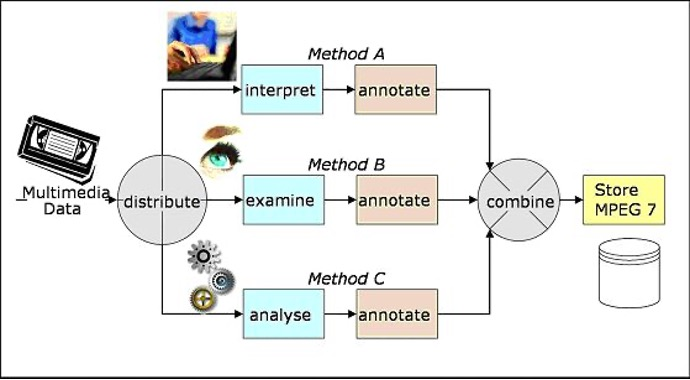
\includegraphics[width=\textwidth]{figure1.jpg}
    \centering
    \captionsetup{font=small}
    \caption{\fontsize{10pt}{11pt}\selectfont{\itshape{Make sure the captions are italics, centred}}}
    \label{fig:1}
\end{figure}

Similar examples of structural complications in version control and
access control Our ma have been discussed at length within the hypermedia and
structural computing communities (e.g., \cite{tois-ver, hoss}).


\subsection{Current status}

There is much ongoing work within the structural computing field (see,
for example, the proceedings of the last three workshops on structural
computing \cite{sc2-proc, sc1-proc, sc3-proc}).  Two modern structural
computing systems are Callimachus \cite{callimachus} and Construct
\cite{construct}....  It is a codebase
successor to three lines of hypermedia research systems --
specifically, DHM \cite{dhm}, HOSS \cite{hoss}, and HyperDisco
\cite{hyperdisco}.  Both the Callimachus and Construct systems
implement a wide variety of structural services.  Recently, a metadata
service, allowing the tagging of WWW pages with arbitrary metadata
records, has been added to Construct \cite{construct-md}.

\section{Metadata as first-class structure}

Metadata is not simply data ...

Secondly, a given metadatum may be related to more than one datum.
For example, two data that share identical authors may both be related
to an identical author metadatum.  This ``transclusion'' \cite{nelson}
model of building metadata references is atypical -- generally, two
metadata records for data that share identical authors simple both
share, for example, identical text in an author key field.  At one
level of abstraction (e.g., the user interface), this model of
metadata may be useful -- a metadata browser may want that matadata
presented as keyword/value pairs.  However, from an implementation
perspective, the keyword/value pair model is a poor choice.  It makes
several types of operations, such as updating information (e.g.,
``change all instances of Joe Public to Joe
Q. Public''), querying for related information (e.g., ``find all
articles authored by Joe Q. Public''), or differentiating
information (e.g., ``which of the three authors named Joe
Q. Public authored this article?'')  unnecessarily difficult...  

\section{Generalized first-class metadata management}

In this section, we present some brief examples of how implementing
metadata management... The implementation and implications of such
examples are described at greater length elsewhere (e.g.,
\cite{tois-ver, hoss}).

\subsection{Data mining}

If metadata are treated as structure ...

\subsection{Adaptive systems}

When structures (both metadata itself, and the structure that binds it
to data) are treated as first-class, they may then be manipulated as
any data object, including being tagged ith attriubute/value pairs and
being versioned.  Both of these characteristics are very useful in
adaptive systems \cite{adapt}...



\section{Conclusions and Future Work}

Until recently, focus in metadata research has focused on what
metadata is and how it should be represented to the user.  However,
there has been a lack of focus on how it should be managed at a system
level.  We have shown that treating metadata as simple data out of the
context of the relationships to which it belongs, and which it
defines, although the current default model, is insufficient.  We
advocate borrowing structure management techniques from fields such as
structural computing to manage metadata more effectively.

\begin{Acknowledgements}
The heading of section ‘Acknowledgement’ must be 10 pt, bold, left justified, with 12pt empty space before and 6pt after. It is absolutely imperative that the references are formatted correctly, i.e. first comes the abbreviation in square brackets, then follows the second name of the author followed by abbreviation of the first name.
\end{Acknowledgements}


\begin{thebibliography}{}{
\fontsize{9pt}{10pt}\selectfont

\bibitem[Anderson and Reich 2000]{sc2-proc} Anderson, K., Reich,
S. (eds.): ``Proceedings of the Second Workshop on Structural Computing''; Lect. Notes Comp. Sci. 1903, Springer, Berlin.

\bibitem[Christodoulakis et~al. 1999]{callimachus} Christodoulakis,
D., Vaitis, M., Papadopoulos, A., Tzagarakis, M.: ``The Callimachus
approach to distributed hypermedia''; Proc. 10$^{th}$ ACM
Conf. Hypert., ACM, New York (Feb 1999).

\bibitem[Gr{\o}nb{\ae}k and Trigg 1994]{dhm} Gr{\o}nb{\ae}k, K.,
Trigg, R.: ``Design issues for a Dexter-based hypermedia system'';
Comm. ACM 37, 2 (Feb 1994), 40-49.

\bibitem[Hicks et~al. 1998]{tois-ver} Hicks, D., Leggett, J.,
N\"{u}rnberg, P., Schnase, J.: ``A hypermedia version control
framework''; ACM Trans. Inf. Sys., 16, 2 (Apr 1998l) 127-160.

\bibitem[LOC 2000]{marc21} Library of Congress: MARC 21 specifications
for record structure, character sets, and exchange media. (2000)
\url{http://www.loc.gov/marc/specifications/spechome.html}.

\bibitem[Marshall et~al. 1994]{viki} Marshall, C., Shipman, F.,
Coombs, J.: ``VIKI: spatial hypertext supporting emergent structure'';
Proc. 1994 Euro. Conf. Hyperm. Tech. (Sep) 13-23.

\bibitem[Martinez 2002]{mpeg7} Martinez, J.: ``Coding of moving
pictures and audio: Overview of the MPEG-7 standard (version 6.0)''
ISO/IEC JTC1/SC29/WG11 N4509 (2001)
\url{http://mpeg.telecomitalialab.com/standards/mpeg-7/mpeg-7.htm}

\bibitem[McCall et~al. 1990]{phidias} McCall, R., Bennett, P.,
D'Oronzio, P., Ostwald, J., Shipman, F., Wallace, N.: ``PHIDIAS:
Integrating CAD graphics into dynamic hypertext''; Proc. 1$^{st}$
Euro. Conf. Hypert. 1990 (Nov), 152-165.

\bibitem[Nelson 1993]{nelson} Nelson, T.: ``Literary Machines'';
Mindful, Sausalito, CA.

\bibitem[Neveu et~al. 2001]{construct-md} Neveu, Y., Guervilly, Y.,
Wiil, U., Hicks, D.: ``Providing metadata services on the World Wide
Web'' Tech. Rep. CSE-01-01, Dept. Comp. Sci. \& Eng, Aalborg
U. Esbjerg, (Mar) \url{http://www.cs.aue.auc.dk/publications}

\bibitem[N{\"{u}}rnberg 1999]{sc1-proc} N\"{u}rnberg, P. (ed.):
``Proceedings of the Workshop on Structural Computing (SC1)''.
Technical Report CSE-99-04, Dept. Comp. Sci. \& Eng., Aalborg
U. Esbjerg, (Feb) \url{http://www.cs.aue.auc.dk/publications}

\bibitem[N{\"{u}}rnberg et~al. 1998]{ecdl} N\"{u}rnberg, P., Wiil, U.,
Leggett, J.: ``Structuring facilities in digital libraries'';
Proc. Euro. Conf. Dig. Lib. 1998 (Sep).

\bibitem[N{\"{u}}rnberg et~al. 1997]{sc} N\"{u}rnberg, P., Leggett,
J., Schneider, E.: ``As we should have thought''; Proc. ACM Hypert.
'97, ACM, New York (1997).

\bibitem[N{\"{u}}rnberg et~al. 1996]{hoss} N\"{u}rnberg, P., Leggett,
J., Schneider, E., Schnase, J.: ``HOSS: a new paradigm for
computing''; Proc. 7$^{th}$ ACM Conf. Hypert, ACM, New York (Mar
1996) 194-202.

\bibitem[Reich et~al. 2001]{sc3-proc} Reich, S., Tzagarakis, M., De
Bra, P. (eds.): ``Proceedings of the Third Workshop on Structural
Computing''; Lect. Notes Comp. Sci. 2266, Springer, Berlin.

\bibitem[Schraefel 2000]{adapt} Schraefel, M.: ``ConTexts: Adaptable
hypermedia"; Proc. Adapt. Hypermedia and Adapt. Web-Based
Sys. Int. Conf., Lect. Notes in Comp. Sci. 1892, Springer, Berlin (Aug
2000), 369-375.

\bibitem[Wiebel et~al. 1998]{dublincore} Weibel, S., Kunze, J.,
Lagoze, C., Wolf, M.: ``Dublin Core metadata for resource discovery'';
IETF RFC 2413 (1998) \url{http://www.ietf.org/rfc/rfc2413.txt}

\bibitem[Wiil and Leggett 1996]{hyperdisco} Wiil, U. Leggett, J.:
``The HyperDisco approach to open hypermedia systems''; Proc. ACM
Conf. Hypert. 1996, ACM, New York (Mar), 140-148.

\bibitem[Wiil and Leggett 1992]{hyperform} Wiil, U. Leggett, J.:
``Hyperform: Using extensibility to develop dynamic, open and
distributed hypertext systems''; Proc. 4$^{th}$ ACM Conf. Hypert.,
ACM, New York (Nov 1992), 251-261.

\bibitem[Wiil and N{\"{u}}rnberg 1999]{construct} Wiil, U.,
N\"{u}rnberg, P.: ``Evolving hypermedia middleware services: Lessons
and observations''; Proc. ACM Symp. Appl. Comp., ACM, New York (Mar
1999).
}\end{thebibliography}


\end{document}
